\chapter{Appendix A: Literature Review Strategy}
\label{cha:anhang_A}

\pagenumbering{arabic} % Reset Page-Numbering to 1
\renewcommand*{\thepage}{A-\arabic{page}} % Nummerierung A-1

The literature review was conducted following a structured methodology, as showcased in \Cref{fig:literature_review}, for comprehensive coverage of all relevant studies.

\begin{figure}[htbp] 
	\centering
	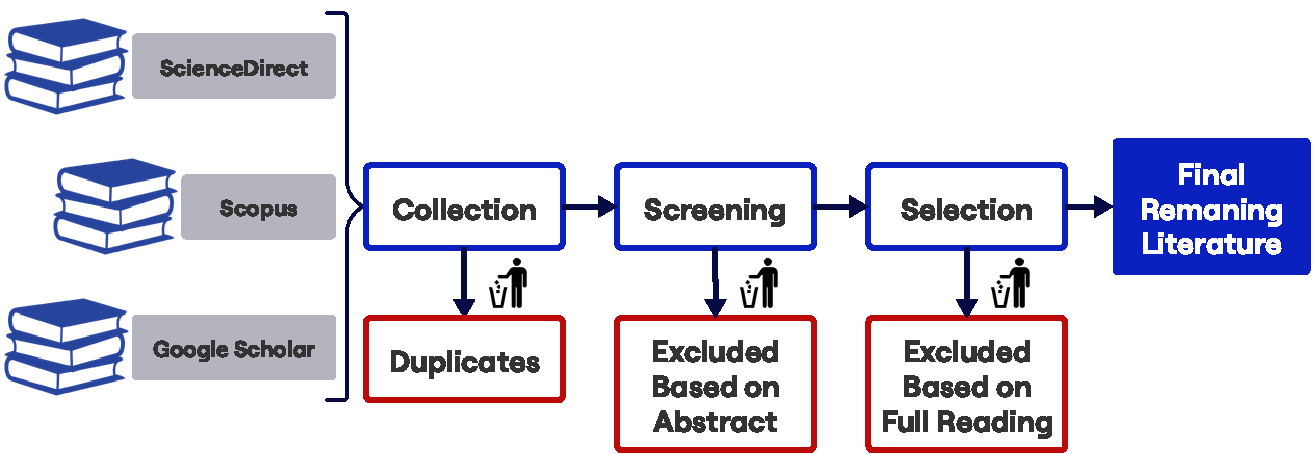
\includegraphics[width=\textwidth]{figures/literature_review.pdf}
    \caption{%
        \textit{Literature Review Strategy}
    }
	\label{fig:literature_review}
\end{figure}

First, an extensive search was performed across multiple academic databases (see \Cref{tab:research_resources}), followed by de-duplication and an initial screening based on titles and abstracts. Articles that passed this screening underwent a full‐text review, ultimately yielding the final set of academic papers aligned with the research objectives.

To capture the breadth of research in the area of \acrlong{dpp}s and their broader ecosystem, both simple keywords and more complex Boolean/phrase combinations were utilized in the search process. \Cref{tab:literature_keyword_search} summarizes the high-level topic categories alongside the respective keyword sets. By incorporating operators such as AND, OR, and quotation marks for exact phrases, the search was optimized to include only the most relevant literature. All of the findings were then imported into Citavi reference management software to streamline organization, elimination, and citation of the reviewed literature. This structured, iterative approach ensured comprehensive coverage and yielded a robust pool of academic sources for the thesis.

\begin{table}[htbp]
  \centering
  \smaller
  \caption{Literature Search Keywords and Boolean Combinations}
  \renewcommand{\arraystretch}{1.2}
    \begin{tabularx}{\textwidth}{|
      >{\arraybackslash}X|
      >{\arraybackslash}X|
      >{\arraybackslash}X|}
      \hline
      \rowcolor{myDarkBlue}\color{white}\textbf{Topic Category} & \color{white}\textbf{Keywords} & \color{white}\textbf{Boolean/Phrase Combinations} \\
      \hline
      DPP Fundamentals & 
        Digital Product Passport, DPP, Product Passport, Battery Passport, DPP system, Digital Passport & 
        (``Digital Product Passport'' OR ``DPP'' OR ``Product Passport'' OR ``Battery Passport'' OR ``DPP System'' OR ``Digital Passport'') \\
      \hline
      Circular Economy \& Regulatory Requirements & 
        Circular Economy, CE, Sustainability, Recycling, Remanufacturing, Extended Producer Responsibility, ESPR, Regulation, Directive & 
        (``Digital Product Passport'' OR ``DPP'') AND (``Circular Economy'' OR ``CE'' OR ``Sustainability'' OR ``Recycling'' OR ``Remanufacturing'' OR ``Extended Producer Responsibility'' OR ``ESPR'' OR ``Regulation'' OR ``Directive'') \\
      \hline
      Technology & 
        Blockchain, Distributed Ledger technology, DLT, Smart Contracts, Verifiable Credentials, Decentralization;
        Digital Twin, Asset Administration Shell, AAS;
        Cloud Computing, Cloud-Native, Microservices, Containerization, Docker, Kubernetes;
        IoT, Sensors, Edge Computing, Predictive Maintenance; Knowledge Graph, Semantic, Ontology & 
        (``Digital Product Passport'' OR ``DPP'') AND ((``Blockchain'' OR ``Distributed Ledger Technology'' OR ``DLT'') AND (``Smart Contracts'' OR ``Verifiable Credentials'' OR ``Decentralization'') OR (``Digital Twin'' OR ``Asset Administration Shell'' OR ``AAS'') OR (``Cloud Computing'' OR ``Cloud-Native'' OR ``Microservices'' OR ``Containerization'' OR ``Docker'' OR ``Kubernetes'') OR (``IoT'' OR ``Sensors'' OR ``Edge computing'' OR ``Predictive Maintenance'') OR (``Knowledge Graph'' OR ``Semantic'' OR ``Ontology'')) \\
      \hline
      Functional \& System Requirements & 
        Requirements, System Requirements, Data, Lifecycle Data, Identifier, Data Carrier, Functionality, Encryption, Security & 
        (``Digital Product Passport'' OR ``DPP'') AND (``Requirements'' OR ``System Requirements'' OR ``Data'' OR ``Lifecycle Data'' OR ``Identifier'' OR ``Data Carrier'' OR ``Functionality'' OR ``Encryption'' OR ``Security'') \\
      \hline
      Implementation \& Adoption & 
        Pilot, Implementation, Case Study, Adoption, Scalability, Deployment, Integration, Best Practices & 
        (``Digital Product Passport'' OR ``DPP'') AND (``Pilot'' OR ``Implementation'' OR ``Case Study'' OR ``Adoption'' OR ``Scalability'' OR ``Deployment'' OR ``Integration'' OR ``Best Practices'') \\
      \hline
      Governance \& Interoperability & 
        Governance, Interoperability, API, Access Control, RBAC, Role-Based, ABAC, Standardization, Federated, Decentralized, Multi-Stakeholder & 
        (``Digital Product Passport'' OR ``DPP'') AND (``Governance'' OR ``Interoperability'' OR ``API'' OR ``Access Control'' OR ``RBAC'' OR ``Role-Based'' OR ``ABAC'' OR ``Standardization'' OR ``Federated'' OR ``Decentralized'' OR ``Multi-Stakeholder'') \\
      \hline
    \end{tabularx}
  \label{tab:literature_keyword_search}
\end{table}
